\chapter{実装の詳細}

\section{ゲーム環境の実装}
\label{sec:game_impl}
2048は状態からafterstateへの遷移において, 各行~(列)~の変化は独立に考えることができる.
また回転と反転を考慮することで上下左右は等価な盤面変化を起こす.
よって$1$行の全パターンについて, ある一方向を選択したときの遷移先を予め計算しておくで, 全方向に対する盤面全体の遷移を高速に行える.

\section{完全解析の実装}
図~\ref{fig:symmtric_boards}に示すように, 回転・反転に関して同じ盤面は$1$つの状態として扱った.
またそれぞれの状態は$64$ビット整数で表現された.
\begin{figure}[t]
    \centering
    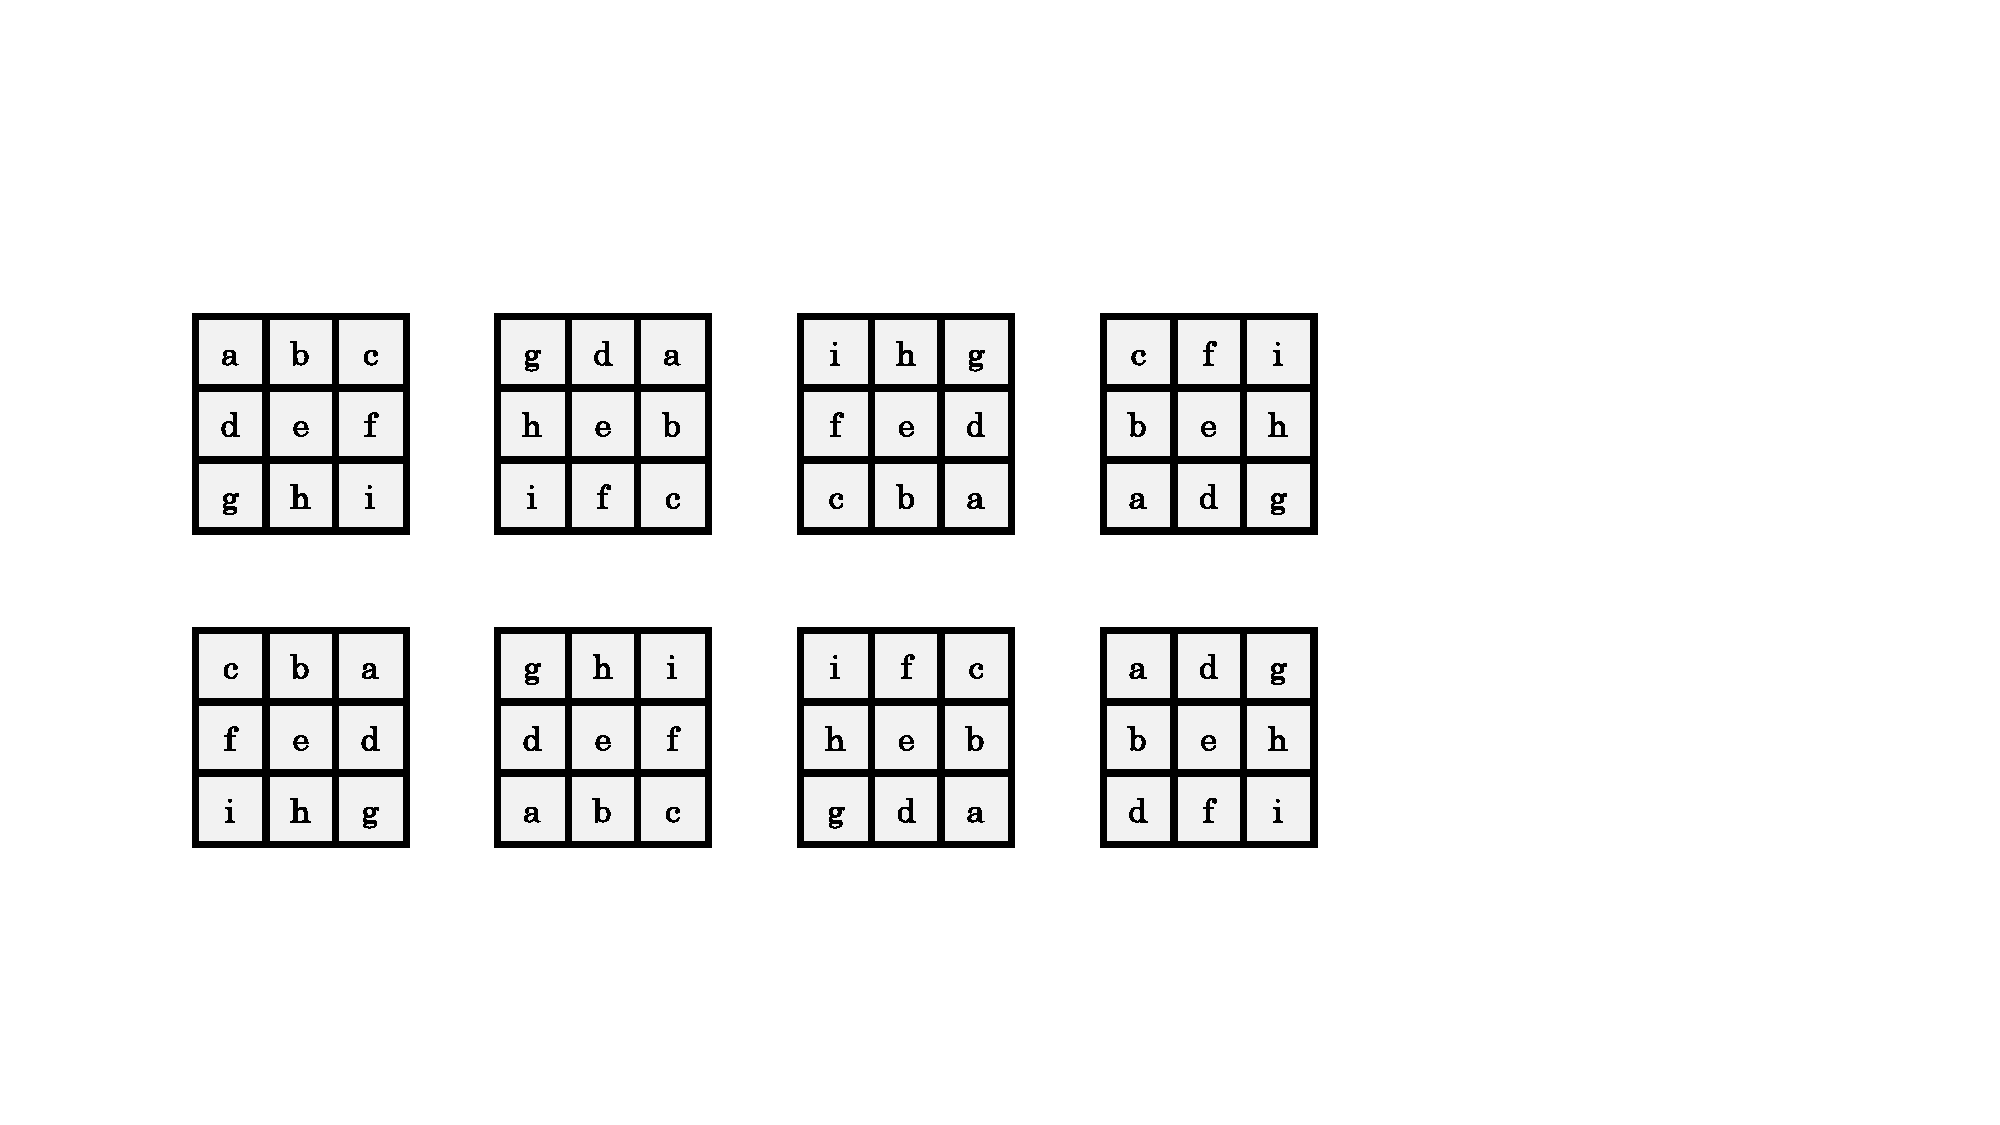
\includegraphics[width=0.6\linewidth{}]{figures/symmetric.pdf}
    \caption{$3\times3$盤面の2048の対称盤面}
    \label{fig:symmtric_boards}
\end{figure}
完全解析にはメモリ$256$GBでプロセッサはコア数$32$のAMD Ryzen Threadripper 3970Xのマシンを用いた.
プログラムはすべてC++言語で実装された.

$4\times3$盤面の2048の完全解析は状態列挙に約$45$日, 価値計算に約$20$日を要した.
ただし実装の細かい工夫の仕方で改善することができると考えられる.
また列挙した状態とその価値の情報を保持するために合計で$16.8$TBの記憶領域を必要とした.
本研究では状態を表す$64$ビットと, 価値を表す$64$ビットを素朴に並べることでデータを記録した.
簡潔データ構造によりデータを圧縮し, より使いやすいデータベースにすることは今後の課題としたい.

\section{強化学習の実装}
\subsection{ニューラルネットワークの詳細}
\label{subsec:nn_impl}
2048-AlphaZeroのニューラルネットワークは盤面の特徴量を入力として, 方策と価値を出力する.
盤面サイズ$H \times W$のルールの下では理論上の最高到達タイルは$2^{H \times W + 1}$である.
そのため入力は空きマスのチャネルを加えた$H \times W + 2$チャネルの$H \times W$ピクセルから成る.
$n$番目~($0 \leq n \leq H \times W + 1$)~のチャネルの$(i,j)$成分は, 盤面の$i$行$j$列目のタイルが$2^n$である場合に$1$, そうでなければ$0$である.
ただし$0$番目のチャネルは空きマスに関する情報を保持する.
図~\ref{fig:input_encoding}に$4\times4$盤面の状態をニューラルネットワークへの入力特徴量に変換する具体例を示す.
\begin{figure}[t]
    \centering
    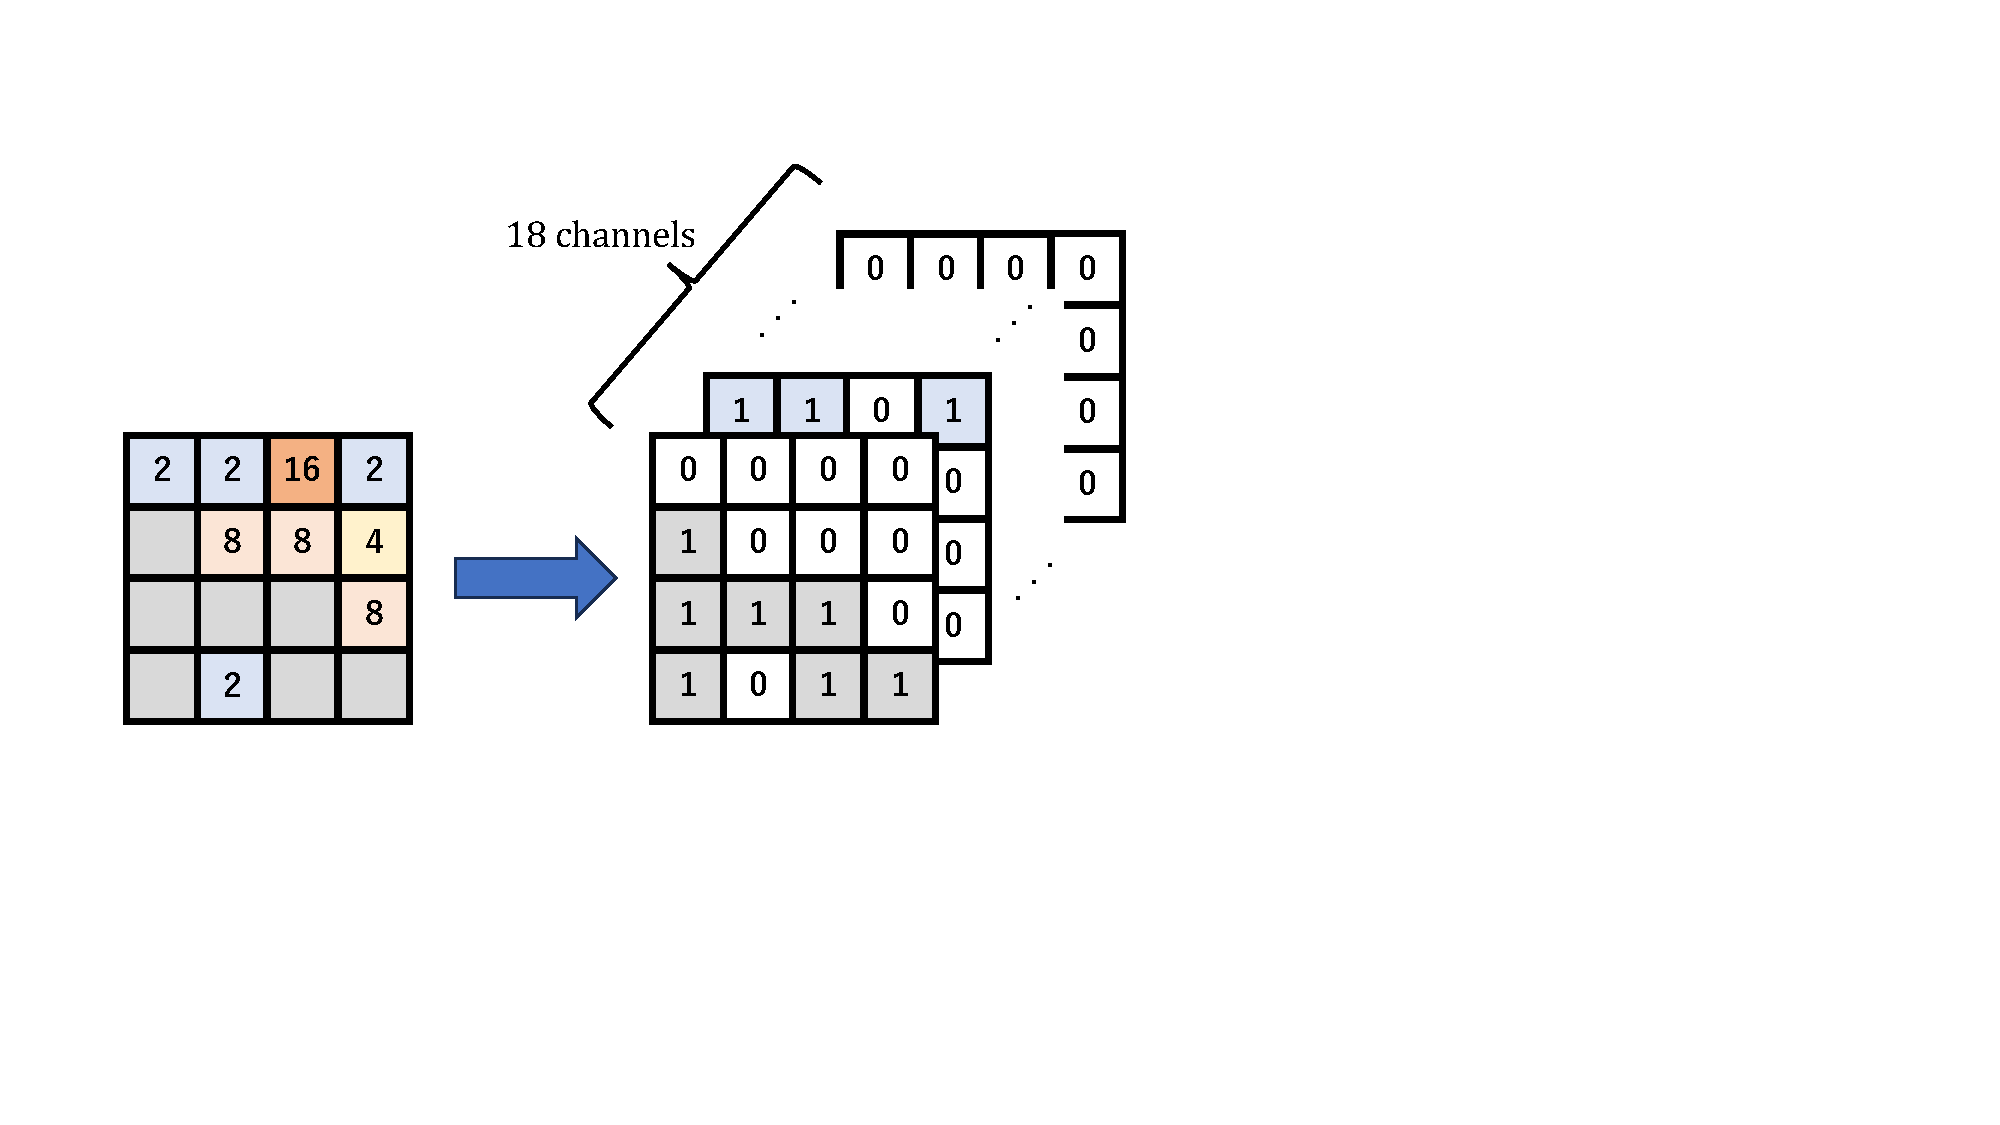
\includegraphics[width=0.6\linewidth{}]{figures/encoding.pdf}
    \caption{ニューラルネットワークへの入力特徴量}
    \label{fig:input_encoding}
\end{figure}

またStochastic MuZero~\cite{StochasticMuZero}に倣って, ニューラルネットワークは価値を$D$次元のベクトル値として出力する.
価値の学習ターゲット$x$~(スカラー値)~は, まず$h(x)= \sqrt{x+1} - 1 + \epsilon x \ (\epsilon=0.001)$によってスケールを調整する~(図~\ref{fig:transform}を参照).
\begin{figure}[t]
    \centering
    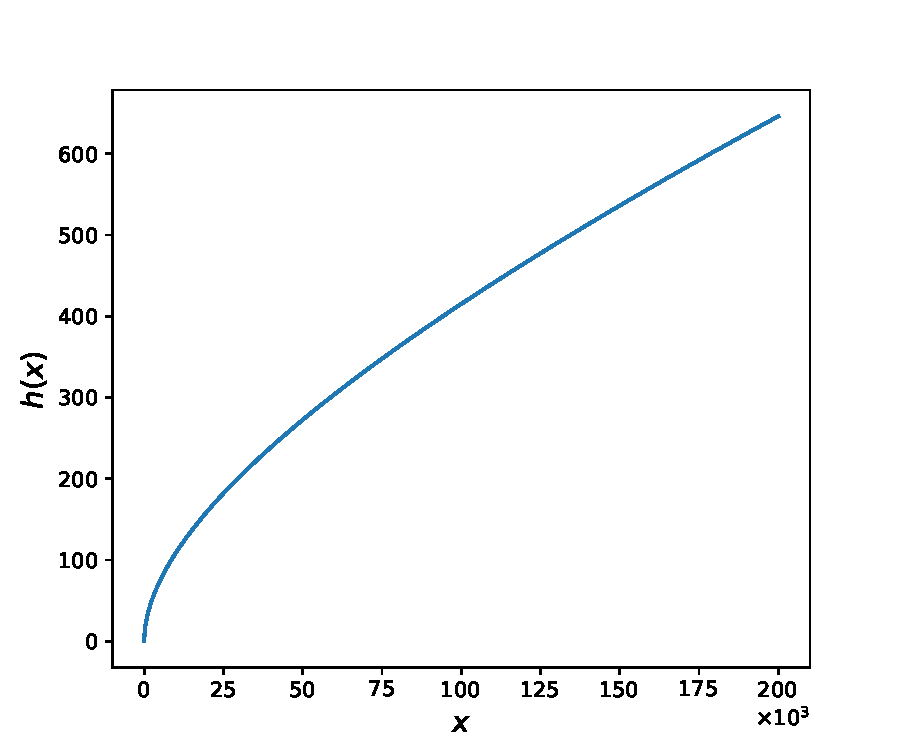
\includegraphics[width=0.6\linewidth{}]{figures/transform_.pdf}
    \caption{$h(x)$のグラフ}
    \label{fig:transform}
\end{figure}
さらに$h(x)$はtwo-hotという, 特定の$2$つの要素以外は全ての$0$であるようなベクトル値に変換される.
たとえば$h(x)=3.7$の場合, $3.7=3 \times 0.3 + 4 \times 0.7$であるため, $3$の重みが$0.3$, $4$の重みが$0.7$, それ以外は$0$である$D$次元ベクトルに変換される.
これをニューラルネットワークの価値の学習ターゲットとして, Cross Entropy誤差を最小化するように訓練される.
推論時にはニューラルネットワークの価値のロジットの出力を, softmaxを通して全体の総和を$1$にする.
これを$0$から$D$までのそれぞれの重みとして, 重み付け平均$y$を計算する.
最後に$h(x)$の逆関数である$h^{-1}(y)= \epsilon^{-1} (y + 0.5\epsilon^{-1} + 1.0) - 0.5 \sqrt{4.0 \epsilon^{-3} y + 1.004 \epsilon^{-4}}$によって, $x=h^{-1}(y)$を得る.
$3\times3$盤面の2048の実験では$D=200$, $4\times3$盤面では$D=400$, $4\times4$盤面では$D=600$とした.

\subsection{Prioritized Experience Replayの実装}
Prioritized Experience Replay~\cite{prioritized}は学習に使用するデータを一様ランダムではなく, priorityと呼ばれる重みに従ってサンプルするExperience Replayである.
$i$番目のデータのpriorityを$p_i$とする.
このとき$i$番目のデータはハイパーパラメータ$\alpha$を用いて, 確率$P(i) = \frac{p_{i}^{\alpha}}{\Sigma_k p_{k}^{\alpha}}$でサンプルされる.

Prioritized Experience Replayからのデータのサンプル, およびpriorityの更新は, sum-treeという二分木でデータを管理することで$\mathcal{O}(\log n)$で行うことができる.
sum-treeの葉ノードはpriorityの値を保持し, 各ノードは左右の子ノードの合計値を保持する.
そのため根ノードはpriority全体の合計値$S$を持つ.
サンプルする際には, まず$0$から$S$までの値をランダムに生成し, 根ノードから葉ノードに至るまでたどることで選ぶ.
図~\ref{fig:sumtree}にsum-treeと具体的なサンプルの仕方を例示する.
\begin{figure}[t]
    \centering
    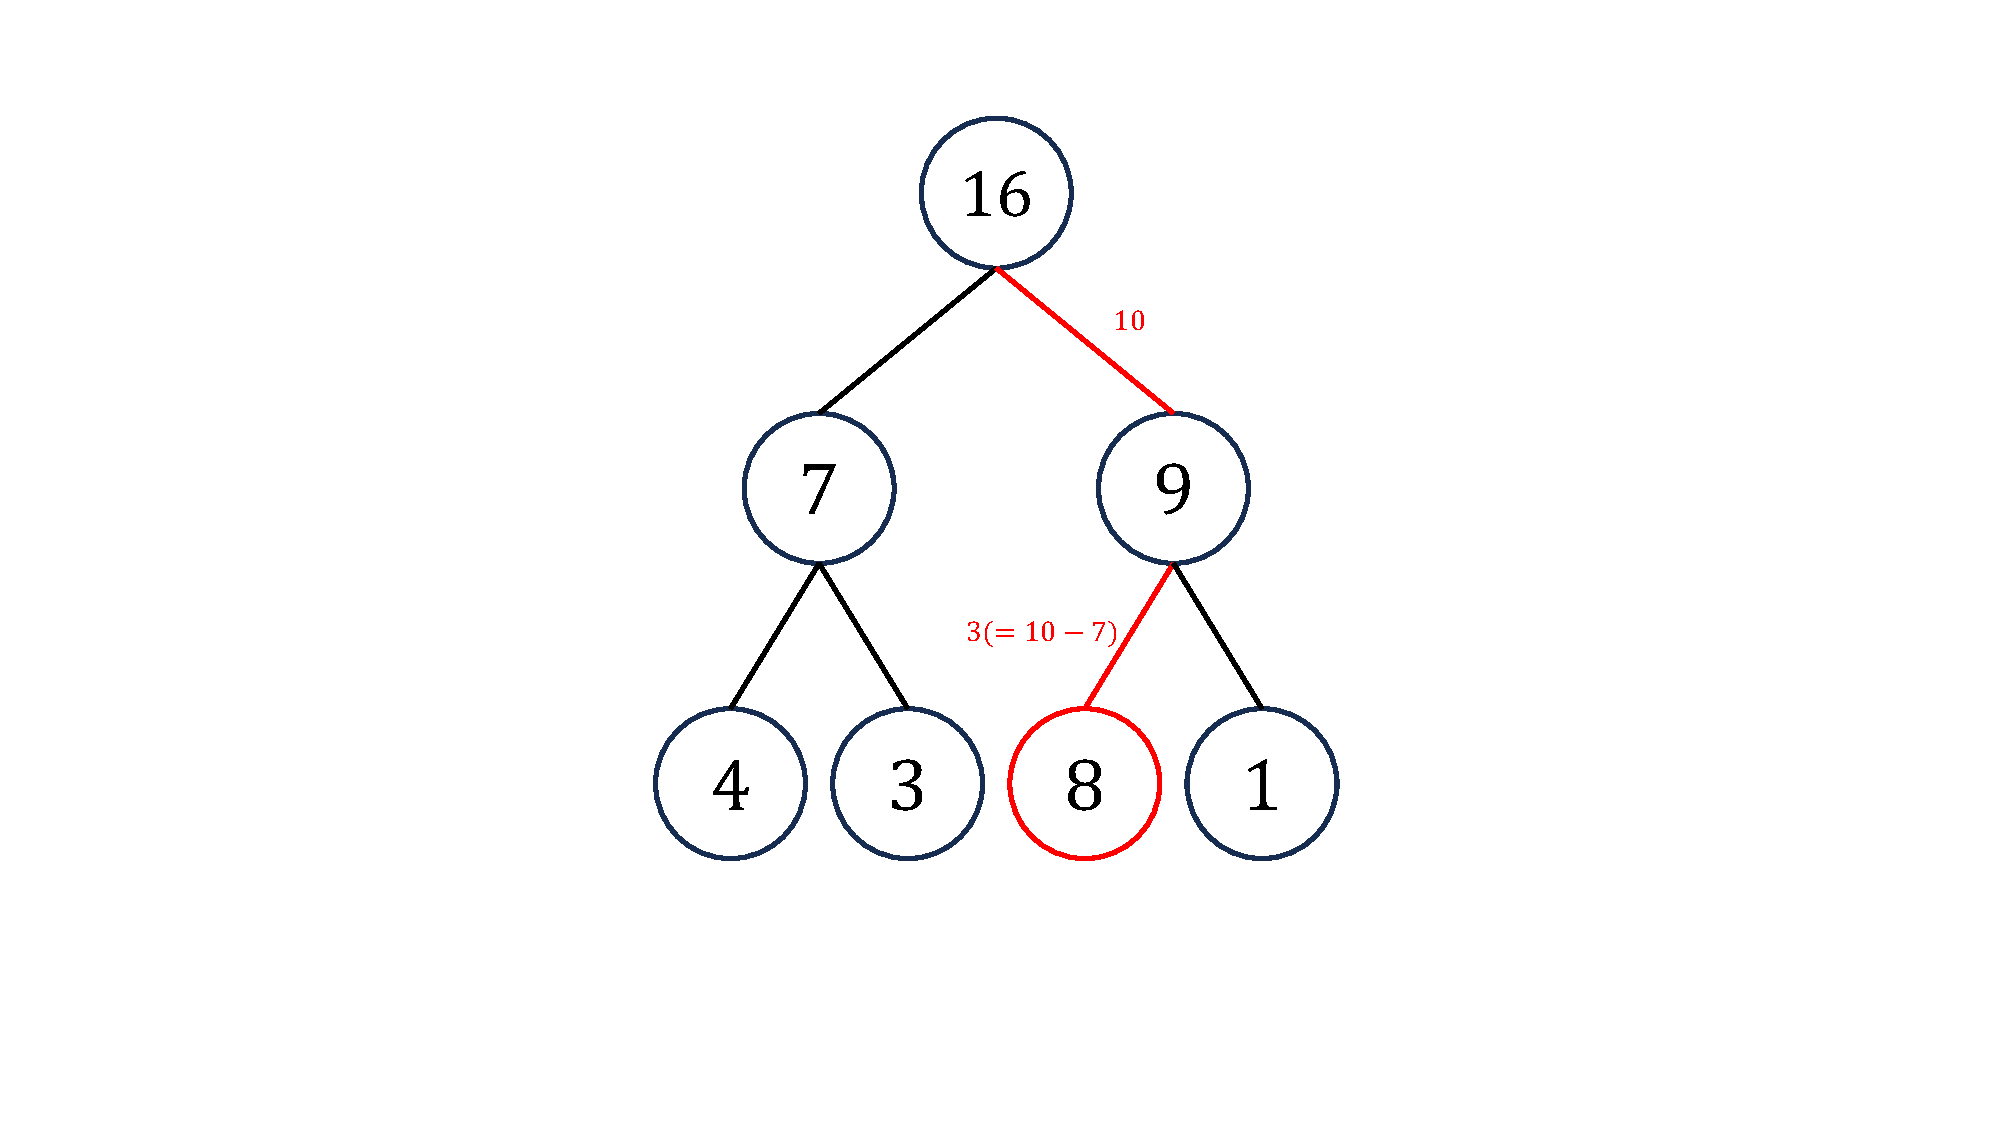
\includegraphics[width=0.4\linewidth{}]{figures/sumtree_.pdf}
    \caption{sum treeの例}
    \label{fig:sumtree}
\end{figure}

\chapter{2048のゲーム性とプレイヤの戦略の検証}
ここでは$3\times3$盤面の2048を主な題材として, 2048のゲーム性とプレイヤの戦略について様々な面から検証する.

\section{2と4の出現確率とプレイヤの得点}
\ref{sec:rule}節で述べたように, 2048の通常のルールではafterstateが次の状態へ遷移する際に出現する, 新しいタイルの数字と位置はランダムに決まる.
すなわちafterstateの空きマスから等確率に選択されたある1マスに$90\%$の確率で$2$のタイルが, $10\%$の確率で$4$のタイルが置かれる.

ここで$2$のタイルと$4$のタイルの出現確率を変更した場合にゲーム性がどう変わるか検証する.
表~\ref{table: value_table}に$3 \times 3$盤面の2048において, $4$の出現確率を通常の$10\%$から増減させたときの完全解析の結果を示す.
表から分かるように, $2$と$4$の出現確率がいずれか一方に傾くほど期待値は大きくなる傾向があることが分かる.
また$4$の出現確率が$0\%$の場合と$100\%$の場合には, 最適な行動をし続ければ常に~図\ref{fig:limit}のような理論上の最終盤面に到達できることが分かる.
2048は$2$と$4$の$2$種類の数字タイルが良い割合で出現することが, 人間がプレイするにあたってゲームを面白くしていると考えられる.
\begin{table}[t]
\caption{4の出現確率を増減させたときのゲームの期待値}
\label{table: value_table}
\centering
\begin{tabular}{r|r||r|r}
    \hline \hline
    4の確率 & 初期状態の期待値 & 4の確率 & 初期状態の期待値 \\ \hline 
    0.00 & 7172.00 & 0.55 & 3206.00 \\
    0.05 & 6161.17 & 0.60 & 3171.24 \\
    \textbf{0.10} & \textbf{5468.49} & 0.65 & 3165.36 \\
    0.15 & 4932.54 & 0.70 & 3194.44 \\
    0.20 & 4515.42 & 0.75 & 3269.18 \\
    0.25 & 4182.44 & 0.80 & 3399.20 \\
    0.30 & 3919.20 & 0.85 & 3607.78 \\
    0.35 & 3704.44 & 0.90 & 3993.30 \\
    0.40 & 3531.46 & 0.95 & 4938.20 \\
    0.45 & 3390.19 & 1.00 & 14344.00 \\
    0.50 & 3278.70 &  & \\
    \hline
\end{tabular}
\end{table}

\section{2048とminmax法}
環境が常にプレイヤにとって最も都合の悪くなるように, 新しい数字タイルを出現させるゲームを考える.
これは二人零和有限完全確定情報ゲームと同様に, minmax法によって完全解析を行える.
よって本稿ではこの場合の環境をminmax環境と呼ぶことにする.
minmax環境の2048は, 得点を最大化したいプレイヤと得点を最小化したい環境の対戦ゲームのように考えることができるため, 「対戦型2048」とも呼ばれている~\cite{battle_2048}.
minmax環境における状態の価値$v_{\text{minmax}}$は, 以下の式~\ref{eq:minmax}に従って, ~\ref{sec:solving}節と同様に後退解析を行い計算できる.
\begin{align}
    v_{\text{minmax}}(s) =
    \begin{cases}
        0 & (s \text{が終了状態}) \\
        \max_a \left(r(s,a) + \min_{s_\text{next} \in \mathcal{T}(s,a)} v_{\text{minmax}}(s_\text{next}) \right) & (\text{otherwise})
    \end{cases}
    \label{eq:minmax}
\end{align}

$3\times3$盤面のminmax環境におけるプレイヤと環境の最善手順を図~\ref{fig:minmax_env}に示す.
ゲームは$21$手で終了し, プレイヤは$164$点しか獲得することができない.
環境がプレイヤの妨害をすると, プレイヤの得点は最善手を選んだとしてもごく僅かになることがわかる.
そのため対戦型2048において環境がプレイヤにとって最悪手を選択する場合, 通常の2048と比べてプレイヤ視点でのゲーム性に欠けるだろう.
対戦型2048に良いゲーム性を持たせるには, 環境側に何らかの制約を加えるなどの工夫をする必要があると考えられる.
\begin{figure}[t]
    \centering
    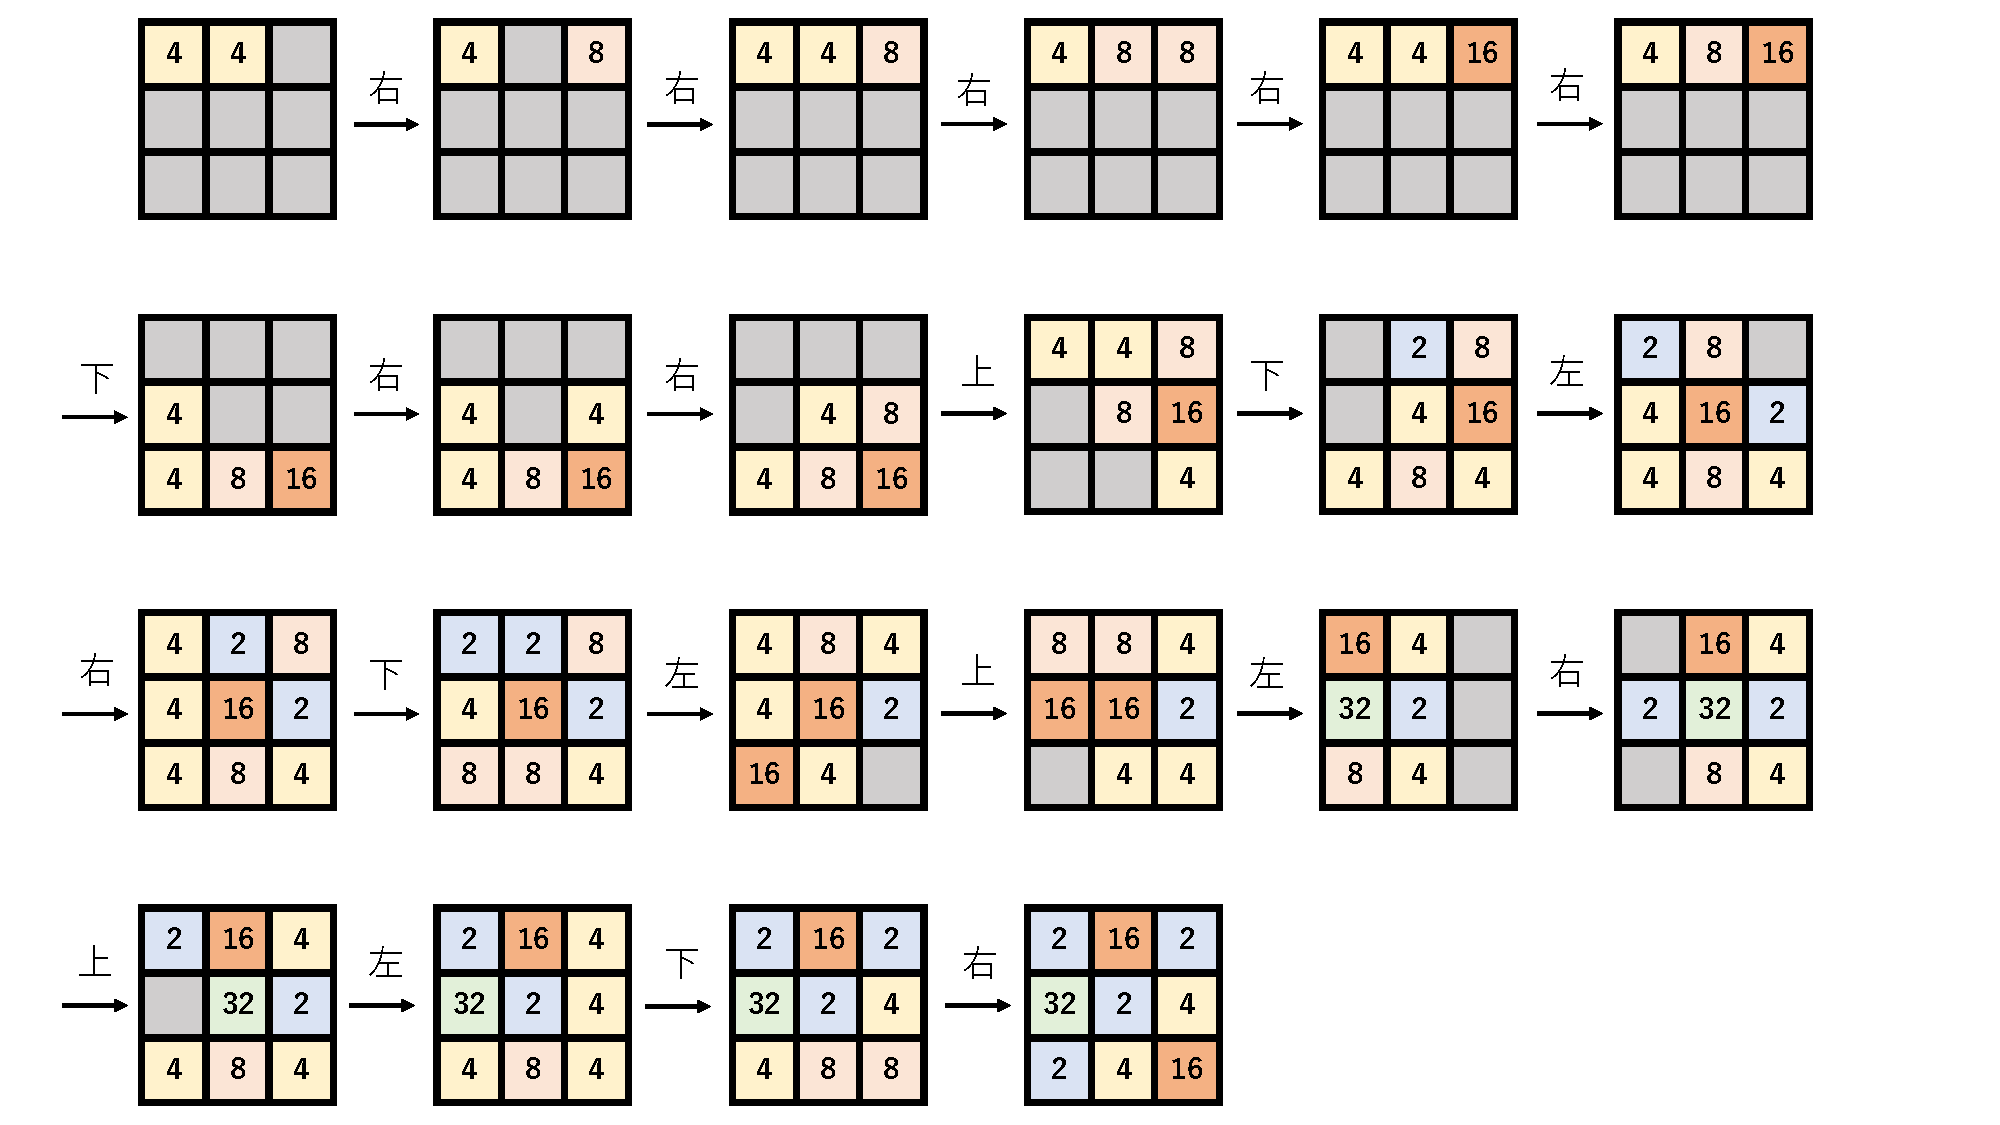
\includegraphics[width=\linewidth{}]{figures/minmax_transition.pdf}
    \caption{$3\times3$盤面のminmax環境における双方の最善手順}
    \label{fig:minmax_env}
\end{figure}

minmax環境と同様に, 環境がプレイヤの得点を最大化させるように振る舞うようなゲームを考えることもできる.
これは式~\ref{eq:minmax}中の$\min$を$\max$に置き換えることで完全解析を行える.
よってこの場合の環境をmaxmax環境と呼ぶことにする.
直感的にも明らかなように, maxmax環境では必ず図~\ref{fig:limit}に示したような理論上の最大盤面に到達することができる.
そのため$3\times3$盤面ではプレイヤは$16,352$点を獲得することができる.

さらに$v_{\text{minmax}}$や$v_{\text{maxmax}}$を評価関数として, 通常のルールの環境でプレイさせることを考える.
それぞれminmaxプレイヤ, maxmaxプレイヤと呼ぶことにする.
minmaxプレイヤが通常のルールの環境で獲得する得点の期待値を$v_{\text{minmax-eval}}$とする.
$v_{\text{minmax-eval}}$は, 以下の式~\ref{eq:minmax_eval}に従って後退解析を行い計算できる.
ただし$a_{\text{minmax}}$を, $v_{\text{minmax}}$を評価関数としたときに選択する行動とする.
\begin{align}
    v_{\text{minmax-eval}}(s) =
    \begin{cases}
        0 & (s \text{が終了状態}) \\
        r(s, a_{\text{minmax}}) + \mathbb{E}_{s_\text{next} \in \mathcal{T}(s, a_{\text{minmax}})} v_{\text{minmax-eval}}(s_\text{next}) & (\text{otherwise})
    \end{cases}
    \label{eq:minmax_eval}
\end{align}
maxmaxプレイヤが通常のルールの環境で獲得する得点の期待値$v_{\text{maxmax-eval}}$についても, 同様に計算できる.

初期状態の$v_{\text{minmax-eval}}$は$1,363.44$点, $v_{\text{maxmax-eval}}$は$429.09$点であった.
minmaxプレイヤは常に最悪な場合を想定して行動を選択する, 保守的な戦略をとるプレイヤといえる.
ゲームオーバーにつながるような行動を避ける一方で, チャンスも逃し続けてしまうため$v_*$に従って行動を選択する場合に比べて獲得できる得点も大きく減少する.
maxmaxプレイヤは常にプレイヤに都合の良い場合を想定して行動を選択する, ギャンブル的な戦略をとるプレイヤといえる.
積極的にチャンスを狙う一方で, 環境の確率を無視した楽観的すぎる行動の選択によりminmaxプレイヤよりも大きく期待得点は小さい.